\documentclass[a4paper,oneside,12pt]{article}
\usepackage[portuguese]{babel}
\usepackage{graphicx}
\usepackage{listings}
\usepackage{indentfirst}

\usepackage{tabularx}
\usepackage{multirow}

\usepackage{xcolor}

\definecolor{codegreen}{rgb}{0,0.6,0}
\definecolor{codegray}{rgb}{0.5,0.5,0.5}
\definecolor{codepurple}{rgb}{0.58,0,0.82}
\definecolor{backcolour}{rgb}{0.95,0.95,0.92}

\lstdefinestyle{mystyle}{
    backgroundcolor=\color{backcolour},   
    commentstyle=\color{codegreen},
    keywordstyle=\color{magenta},
    numberstyle=\tiny\color{codegray},
    stringstyle=\color{codepurple},
    basicstyle=\ttfamily\footnotesize,
    breakatwhitespace=false,         
    breaklines=true,                 
    captionpos=b,                    
    keepspaces=true,                 
    numbers=left,                    
    numbersep=5pt,                  
    showspaces=false,                
    showstringspaces=false,
    showtabs=false,                  
    tabsize=2
}

\lstset{style=mystyle}

\linespread{1.5}

\usepackage{fontspec}
\setmainfont{Times New Roman}

\title{Formato Bitmap}
\author{Canoi Gomes}
\date{23 de Junho de 2024}

\begin{document}
\maketitle
\newpage
\tableofcontents
\newpage
\section{Introdução}

No texto anterior eu dei uma rápida explicação sobre como funciona um arquivo binário, como construir o seu próprio e fazer um programa para escrever e ler.

O formato de arquivo bitmap (possui a extensão \textbf{.bmp}) é um formato normalmente utilizado para guardar os dados de pixel de uma image. É um dos formatos que são conhecidos por geralmente não ter compressão, então diferente de um .png, onde existe um algoritmo de compressão para codificar e decodificar, resultando em um arquivo com tamanho menor. Já no bitmap não, nós conseguimos calcular exatamente qual será o tamanho do arquivo, se temos uma image 24x24 com pixels RGB (ou seja, meu pixel é representado por 3 bytes, 1 para cada canal), nós podemos fazer o seguinte para determinar o tamanho do arquivo:

\noindent
$
24 * 24 = 576\\
576 * 3 = 1728
$

Ou seja, nosso arquivo terá por volta de 1.7 kb, isso desconsiderando o cabeçalho.

\section{Cabeçalho}

O formato bitmap possui dois cabeçalhos, um \textbf{cabeçalho de arquivo} e um \textbf{cabeçalho de informação}. O de arquivo tem 14 bytes, e o de informação de 40 bytes.

\begin{figure}[ht]
    \centering
    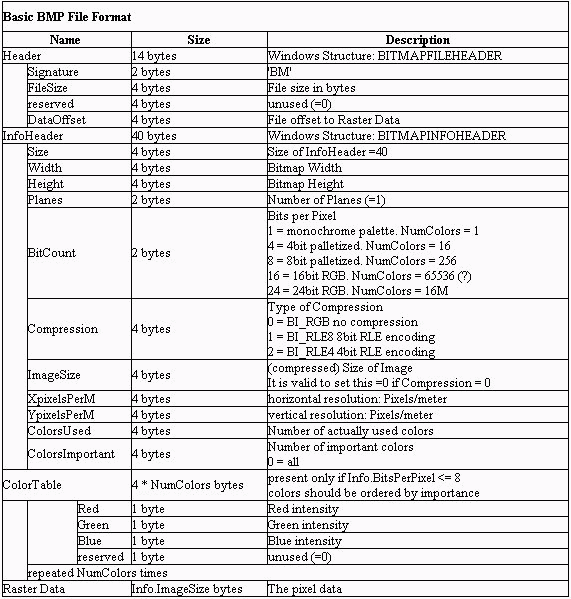
\includegraphics[width=\linewidth]{media/bmp_header.png}
\end{figure}
\break

\subsection{Cabeçalho de Arquivo}

O cabeçalho de arquivo possui 14 bytes de tamanho, como descrito na imagem acima:

\begin{center}
\begin{tabular}{|p{0.2\linewidth}|p{0.1\linewidth}|p{0.6\linewidth}|}
    \hline
    Validação & \textbf{2 bytes} & É usado para a validação do formato, seria seu magic number, geralmente é preenchido com "BM".\\
    \hline
    Tamanho & \textbf{4 bytes} & Tamanho do arquivo em bytes.\\
    \hline
    Reservado & \textbf{4 bytes} & Geralmente não é utilizado.\\
    \hline
    Offset & \textbf{4 bytes} & A partir de onde podemos começar a ler os dados dos pixels do arquivo. Em uma imagem padrão, que não tenha informações extra antes dos pixels, esse valor é 54 geralmente, que seria a soma dos valores de ambos os cabeçalhos (14 + 40).\\
    \hline
\end{tabular}
\end{center}

Poderia representá-lo assim em C.
\begin{lstlisting}[language=C, caption=Cabeçalho de Arquivo em C]
struct FileHeader {
    char magic[2];
    char size[4];
    char reserved[4];
    char offset[4];
};
\end{lstlisting}

\subsection{Cabeçalho de Informação}

O cabeçalho de informação tem 40 bytes de tamanho, e é nele que geralmente vão as informações relativas a imagem como sua paleta de cores, a quantidade de bits que estou usando para representar um pixel, as dimensões, entre outras coisas.
\begin{center}
\begin{tabular}{|p{0.2\linewidth}|p{0.1\linewidth}|p{0.6\linewidth}|}
    \hline
    \textbf{Campo} & \textbf{Bytes} & \textbf{Descrição} \\
    \hline
    Tamanho do Cabeçalho & \textbf{4 bytes} & Aqui irá conter o tamanho do cabeçalho em bytes, geralmente esse valor será 40 mesmo.\\
    \hline
    Largura & \textbf{4 bytes} & Largura da imagem\\
    \hline
    Altura & \textbf{4 bytes} & Altura da imagem\\
    \hline
    Planos & \textbf{2 bytes} & Número de planos (também não sei para que serve, geralmente é 1)\\
    \hline
    Bits Por Pixel & \textbf{2 bytes} & Esse campo é interessante, nele eu especifico a quantidade de bits que quero usar para representar um pixel. É comum esse valor ser 24 (RGB com 3 bytes, ou seja 1 byte para cada canal) ou 32 (RGBA com 4 bytes). Porém também pode ser 16 (também é RGB, mas é um RGB565, 5 bits para R, 6 para G e 5 para B). Se setarmos valores abaixo de 16, como 8 ou 4, precisamos especificar uma paleta de cores logo depois do cabeçalho. 8 bits por exemplo, preciso de uma paleta com 256 cores, 4 bits uma paleta com 16 cores e assim vai.\\
    \hline
    Compressão & \textbf{4 bytes} & Aqui basicamente você pode setar um modo de compressão, mas como não estamos utilizando nenhum geralmente esse valor será zero mesmo.\\
    \hline
    Tamanho da Imagem & \textbf{4 bytes} & Aqui vai representar o tamanho da imagem após a compressão. Se não tiver nenhum compressão, como é o nosso caso, esse valor pode ser zero também.\\
    \hline
    
\end{tabular}
\end{center}

\begin{center}
\begin{tabular}{|p{0.2\linewidth}|p{0.1\linewidth}|p{0.6\linewidth}|}
    \hline
    XpixelsPerM & \textbf{4 bytes} & \\
    \hline
    YpixelsPerM & \textbf{4 bytes} & \\
    \hline
    Cores Usadas & \textbf{4 bytes} & \\
    \hline
    Cores Importantes & \textbf{4 bytes} & \\
    \hline
\end{tabular}
\end{center}

Posso representar esse cabeçalho assim em C:
\begin{lstlisting}[language=C, caption=Cabeçalho de Informação em C]
struct InfoHeader {
    char header_size[4];
    char width[4];
    char height[4];
    char planes[2];
    char bits_per_pixel[2];
    char compression[4];
    char image_size[4];
    char x_pixels[4];
    char y_pixels[4];
    char colors_used[4];
    char colors_important[4];
};
\end{lstlisting}

\end{document}